% Latex file for the MPI Course at HPC2N Umea 
%    Elaborated by P. Ojeda
%
\documentclass{beamer}
%\documentclass[12pt]{article}
%\usepackage{beamerarticle}
\setbeamertemplate{navigation symbols}{}


\usetheme{Warsaw}
\usepackage{xcolor}
%\usepackage{chemmacros}
\usepackage{textpos}
%\usepackage{verbatim}
\usepackage{fancyvrb}
\DefineVerbatimEnvironment{ColorVerbatim}{Verbatim}%
  {formatcom=\color{purple},commandchars=\\\{\}}

%\usepackage[utf8]{inputenc}
%\usepackage[T1]{fontenc}
%\usepackage{lmodern}
\usepackage{listings}
%\usepackage{alltt}

\lstset{language=C,
  basicstyle=\ttfamily,
  keywordstyle=\color{blue}\ttfamily,
  stringstyle=\color{red}\ttfamily,
  commentstyle=\color{teal}\ttfamily,
  morecomment=[l][\color{magenta}]{\#}
}


\newcommand{\hilite}[1]{\colorbox{yellow}{#1}}

\setbeamercovered{invisible}
\beamersetuncovermixins{\opaqueness<1>{25}}{\opaqueness<2->{15}}
\begin{document}
% logo of my university
%\titlegraphic{\vspace*{-5cm} \hspace*{8.75cm} 
\includegraphics[width=1.5cm]{umea_logo.eps}
%}
%\logo{
\includegraphics[width=1.5cm]{umea_logo.eps}
%}

\title{ Introduction to Abisko and Kebnekaise} \author{Pedro Ojeda-May, Jerry Eriksson,
	 and Birgitte Bryds\"{o}
} \institute[Ume\aa University]{
  HPC2N, \\
  Ume\aa University,\\[1em]
\includegraphics[width=0.8cm]{images/umea_logo.eps} \\
  901 87, Sweden.
  }

\date{\today}

% position the logo
\addtobeamertemplate{frametitle}{}{%
\begin{textblock*}{100mm}(\textwidth,-1.6cm)

\includegraphics[height=1cm,width=1cm,keepaspectratio]{images/logo_hpc2n.eps}
\end{textblock*}}

%%%%%%%%%%%%%%%%% NEW  SLIDE
\begin{frame}
	\titlepage
\end{frame}

%%%%%%%%%%%%%%%%% NEW  SLIDE
\begin{frame}
	\frametitle{Table of contents}

	\tableofcontents
\end{frame}



%########################  NEW SECTION  ########################
%% Section: Why?
% Latex file for the MPI Course at HPC2N Umea 
%    Elaborated by P. Ojeda
%

%########################  NEW SECTION  ########################
\section{Why?}



%%%%%%%%%%%%%%%%% NEW  SLIDE
\begin{frame}
	\frametitle{Why?}
  
	\begin{itemize}
		\item	Computations take too long time
			\begin{itemize}
				\item	Use an already parallelized software
				\item	Doing it yourself
					\begin{itemize}
						\item	Doing it yourself\\
								- Run each instance on a separate core\\
								- If inside a loop, maybe suitable for
										simple parallelization
						\item	More complex problems requires more explicit
								parallel programming
					\end{itemize}
			\end{itemize}
		\item	Use your computer for other things
		\item	Requires a lot of memory (up to 256 GB main memory)
		\item	Solve larger (more interesting/realistic) problems
	\end{itemize}

\end{frame}




%########################  NEW SECTION  ########################
%% Section: How to Apply
% Latex file for the MPI Course at HPC2N Umea 
%    Elaborated by P. Ojeda
%

%########################  NEW SECTION  ########################
\section{How to apply}

%------------------  NEW SUBSECTION ------------------
\subsection{Projects}

%%%%%%%%%%%%%%%%% NEW  SLIDE
\begin{frame}[fragile]
	\frametitle{SUPR - SNIC User and Project Repository}
	\begin{enumerate}
		\item	Get a login at SUPR (\texttt{https://supr.snic.se/})
		\item	Create a proposal for a project \\
				{\small  (at least: Title, Abstract, Resource Usage, Classification, length of project (1-12 months), which resource(s) you wish to use, and the amount of core hours/month you need.)}
		\item	Get an account at HPC2N
	\end{enumerate}
  
\end{frame}

%%%%%%%%%%%%%%%%% NEW  SLIDE
\begin{frame}
	\frametitle{Small level requests}
  
	\begin{itemize}
		\item	Max 5000 core hours/month/resource (Abisko)
		\item	Can be submitted at any time (short abstract)
		\item	Applications handled locally at the SNIC centers
		\item	For small projects and new groups that want to
				gain experience in using HPC systems
		\item	The PI must be employed at a Swedish university
				(e.g., PhD student or higher)
	\end{itemize}

\end{frame}

%%%%%%%%%%%%%%%%% NEW  SLIDE
\begin{frame}
	\frametitle{Medium level requests}
  
	\begin{itemize}
		\item	Up to 160000 core hours/month/resource (Abisko)
		\item	Can be submitted at any time
		\item	Applications handled locally at the SNIC centers
				and assesses the feasibility of using the requested recourses
		\item	Evaluated once a month
		\item	The PI must be a senior scientist in Swedish academia
	\end{itemize}

\end{frame}

%%%%%%%%%%%%%%%%% NEW  SLIDE
\begin{frame}
	\frametitle{Large level requests}
  
	\begin{itemize}
		\item	Above the medium level (160000 on Abisko)
		\item	Calls for proposals for large level allocations
				are issued twice a year by SNAC
		\item	Applications are evaluated by SNAC and they also decides on the
				allocations, based on scientific merit, need for the resources,
				efficient use of the resources, and impact
		\item	The PI must be a senior scientist in Swedish academia
	\end{itemize}

\end{frame}


%------------------  NEW SUBSECTION ------------------
\subsection{Accounts}

\begin{frame}
	\frametitle{User Account}

	\begin{itemize}
		\item	Submit an account application using our online form
			\begin{itemize}
				\item	Name and affiliation
				\item	Which project you are taking part in (if any)
				\item	Choose a user name
			\end{itemize}
		\item	Print the final form twice
			\begin{itemize}
				\item	Sign and send one to us together with a copy of
						your passport (do NOT send by email)
				\item	Keep one (your initial password is on it)
			\end{itemize}

	\end{itemize}

\end{frame}




%########################  NEW SECTION  ########################
%% Section: Support
% Latex file for the MPI Course at HPC2N Umea 
%    Elaborated by P. Ojeda
%


%########################  NEW SECTION  ########################
\section{Support}
\begin{frame}
	\frametitle{User Support}

	\begin{itemize}
		\item	\texttt{www.hpc2n.umu.se}
			\begin{itemize}
				\item	Quick-start guides
				\item	How to access, compile, and submit
				\item	Installed software\\
						- Descriptions and how to use them at HPC2N
			\end{itemize}
		\item	\texttt{support@hpc2n.umu.se}
			\begin{itemize}
				\item	Problems
				\item	Requests
			\end{itemize}
	\end{itemize}

\end{frame}

\begin{frame}
	\frametitle{User Support}

\includegraphics[width=10.5cm]{images/web.png}

\end{frame}

\begin{frame}
	\frametitle{User Support}

	\begin{itemize}
		\item	Meetings with individuals or groups
			\begin{itemize}
				\item	To see how can HPC2N be of help
				\item	Help to get started
				\item	Help to parallelize
			\end{itemize}
		\item	HPC2N Think Tank - Open house
		\item	Courses (0.5 - 3 days)
			\begin{itemize}
				\item	Introduction on how to use our system
				\item	Parallel programming (MPI, OpenMP) Oct. 2016
				\item	Computational Chemistry, MD simulations Nov. 2016
			\end{itemize}
	\end{itemize}

\end{frame}




%########################  NEW SECTION  ########################
% Section: Using Abisko
% Latex file for the MPI Course at HPC2N Umea 
%    Elaborated by P. Ojeda
%

%########################  NEW SECTION  ########################
\section{Using Abisko}

%%%%%%%%%%%%%%%%%% NEW  SLIDE
%\begin{frame}
%	\frametitle{Abisko}
%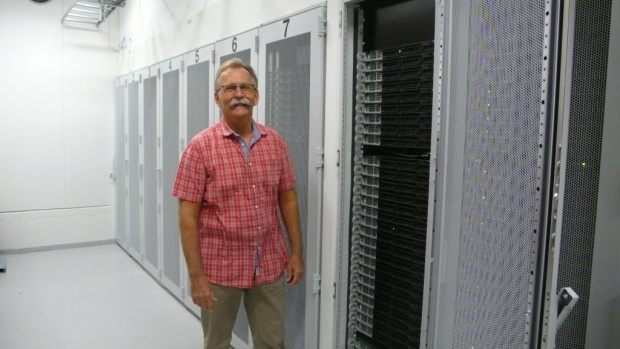
\includegraphics[width=4.5cm]{images/abisko.jpg}
%	\begin{itemize}
%		\item	332 nodes/15936 cores
%		\item	10 fat nodes (512 GB RAM), 318 thin nodes (128 GB RAM)
%		\item	CPUs: (thin) 4 x AMD Opteron 6238 (Interlagos) 12 core (2.6 GHz)
%		\item	CPUs: (fat) 4 x AMD Opteron 6344 (Abu Dhabi) 12 core (2.6 GHz)
%		\item	Interconnect: Infiniband QDR, 40Gb/s, Mellanox
%		\item	Installed 2011
%	\end{itemize}
%\end{frame}
%
%%%%%%%%%%%%%%%%%% NEW  SLIDE
%\begin{frame}
%	\frametitle{Abisko}
%	\begin{itemize}
%		\item	Application software: Abinit, Ansys, DDT, Espresso,
%				Gamess, Gaussian, Gromacs, HDF5, Matlab, NetCDF,
%				NWChem, Octave, PETSc, R, Siesta, VASP, WRF, ...
%		\item	Num. and Comm. libraries: BLACS, FFTW, BLAS, LAPACK,
%				ScaLAPACK, ACML, Intel MKL, ParMETIS, RECSY, SLICOT, ...
%		\item	MPI: OpenMPI, Intel MPI
%		\item	Other software on request
%	\end{itemize}
%\end{frame}
%
%
%%%%%%%%%%%%%%%%%% NEW  SLIDE
%\begin{frame}
%	\frametitle{Kebnekaise}
%\begin{columns}
%	\column[T]{5cm}
%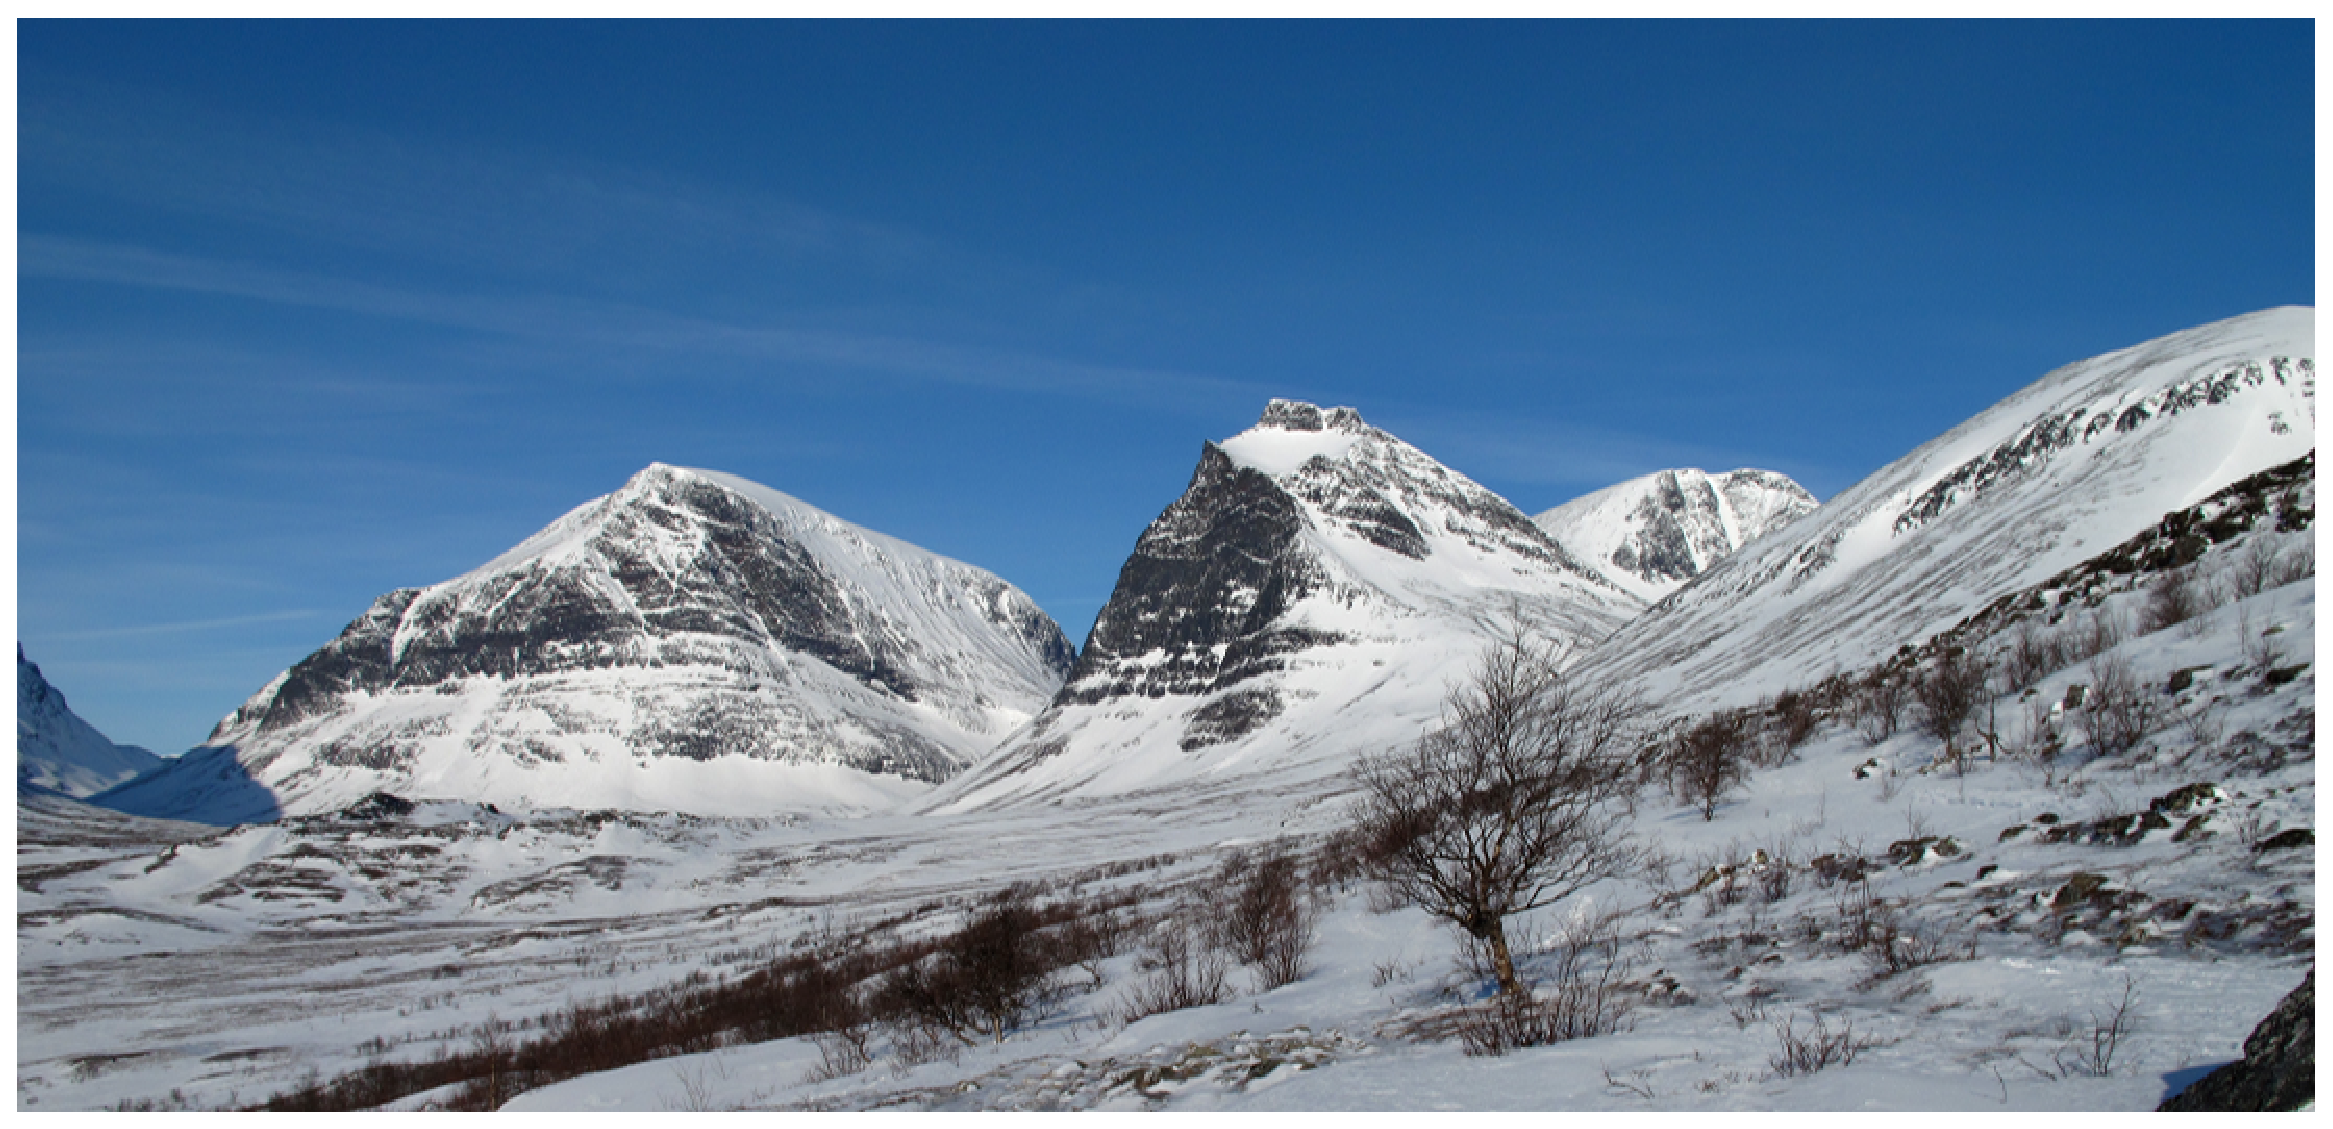
\includegraphics[width=5cm]{images/kebnekaise.eps}
%	\begin{itemize}
%		\item	13 racks, Mixed system:
%		\item	432 Intel Broadwell, E5-2690v4 (2x14 cores/node), 128 GB/node
%		\item	36 Intel Broadwell + NVidia K80 GPUs (32 with 2/node, 4 with 4/node)
%	\end{itemize}
%	\column[T]{5cm}
%	\begin{itemize}
%		\item	20 Intel Haswell E7-4850v3, (4x14 cores/node), 3 TB/node (fat nodes)
%		\item	36 Intel KNL: 7250 SKU (68 cores, 1.4/1.2 Ghz/AVX), 192 GB/node
%		\item	Interconnect: Mellanox Infiniband FDR
%	        \item   OS: Linux Ubuntu
%	        \item   Installation: Summer/Fall 2016
%	\end{itemize}
%\end{columns}
%\end{frame}



%%------------------  NEW SUBSECTION ------------------
%\subsection{Modules}
%
%%%%%%%%%%%%%%%%%% NEW  SLIDE
%\begin{frame}
%	\frametitle{Modules}
%
%	\begin{itemize}
%		\item	Many versions of software packages
%		\item	Use a tool called modules
%			\begin{itemize}
%				\item	Can choose a combination of libraries and compilers
%						that will work together
%				\item	Changes the environment
%				\item	User guide and man-page
%			\end{itemize}
%	\end{itemize}
%
%\end{frame}
%%%%%%%%%%%%%%%%%% NEW  SLIDE
%\begin{frame}
%	\frametitle{Modules}
%
%	\begin{itemize}
%		\item	Some useful module commands
%			\begin{description}
%				\item[help]		list all module commands
%				\item[show]		display information on a module
%				\item[add]		add a module to the environment
%				\item[rm]		remove a module from the environment
%				\item[list]		list currently activated modules
%				\item[avail]	list all modules that exist on the system
%			\end{description}
%		\item	Examples
%			\begin{itemize}
%				\item	\texttt{module add pgi}\\
%						will add the latest version of the Portland compilers
%				\item	\texttt{module add openmpi/pgi}\\
%						will add the latest version of openmpi
%						(suitable for the current machine)
%						that was built with the Portland compilers
%			\end{itemize}
%	\end{itemize}
%
%\end{frame}

%------------------  NEW SUBSECTION ------------------
\subsection{File Systems}

%%%%%%%%%%%%%%%%% NEW  SLIDE
\begin{frame}
	\frametitle{File Systems}


\begin{columns}
	\column[T]{5cm}
		There are 2 file systems\\
		AFS
		\begin{itemize}
			\item	Your home directory (cd \$HOME)
			\item	Backed up regularly
			\item	NOT accessable by the batch system
		\end{itemize}
		PFS
		\begin{itemize}
			\item	Parallel file system
			\item	NO BACKUP
			\item	Accessable by the batch system
		\end{itemize}
	\column[T]{5cm}
		\vspace*{-1cm}
		\includegraphics[width=6.5cm]{images/filesystem.eps}
\end{columns}
\end{frame}

\begin{frame}
    \frametitle{PFS}

	\begin{itemize}
		\item	Offers high performance when accessed from the nodes
		\item	This is the correct place to run all your batch jobs
		\item	To create soft link from your home directory to your
				corresponding home on the parallel file system\\
				\texttt{ln~-s~/pfs/nobackup\$HOME~\$HOME/pfs}
		\item	Then if you use\\
				\texttt{cd pfs}\\
				from your home directory
				you will end up in your "parallel" home directory
				
	\end{itemize}
	
\end{frame}


%------------------  NEW SUBSECTION ------------------
\subsection{Batch System}

%%%%%%%%%%%%%%%%% NEW  SLIDE
\begin{frame}
	\frametitle{Batch System (SLURM)}

	\begin{itemize}
		\item	Large/parallel programs, run through the batch system
		\item	Keeps track of available system resources
		\item	Takes care of scheduling jobs of multiple users,
				running tasks simultaneously
		\item	Enforces local system resource usage and job scheduling policies
		\item	Users submit to a queue (running, idle, blocked)
		\item	Same batch system on  Abisko and Kebnekeise. The differences are that
			there are GPUs and KNLs which can be allocated on Kebnekeise.
		\item   Guides at: http://www.hpc2n.umu.se/support/
	\end{itemize}

\end{frame}


%%%%%%%%%%%%%%%%% NEW  SLIDE
\begin{frame}
	\frametitle{Batch System (SLURM)}

Useful commands:
	\begin{itemize}
		\item	squeue -u $<$username$>$
		\item   srun $<$commands for your job/program$>$
		\item   salloc
		\item   scontrol show job $<$jobid$>$
                \item   scancel $<$jobid$>$
	\end{itemize}

\end{frame}
%%%%%%%%%%%%%%%%% NEW  SLIDE
\begin{frame}[fragile]
	\frametitle{Interactive jobs}

	\begin{verbatim}
	$ salloc -N 1 -n 8 --time=1:30:00 
	\end{verbatim}

It asks to allocate 1 node/8 processors. Once job has been allocated 
we can run our programs

	\begin{verbatim}
	srun -n 2 my_program
	\end{verbatim}

plus additional environment variables if the case.

\end{frame}

%%%%%%%%%%%%%%%%% NEW  SLIDE
\begin{frame}[fragile]
	\frametitle{Job script}
  
\begin{columns}
	\column[T]{5cm}
	\only<1->{\texttt{\#!/bin/bash}\\}
	\only<1,3->{\texttt{\#SBATCH~-A~SNICYYYY-XX-NN}\\}
	\only<2>{\hilite{\texttt{\#SBATCH~-A~SNICYYYY-XX-NN}}\\}

	\only<1-2,5-7,9->{\texttt{\#SBATCH -n 48}\\}
	\only<3-4,8>{\hilite{\texttt{\#SBATCH -n 48}}\\}

	\only<1-4,6->{\texttt{\#SBATCH --time=01:00:00}\\}
	\only<5>{\hilite{\texttt{\#SBATCH --time=01:00:00}}\\}

	\only<1->{\texttt{ }\\}

	\only<1-5,7,9->{\texttt{module add openmpi/gcc}\\}
	\only<6,8>{\hilite{\texttt{module add openmpi/gcc}}\\}

	\only<1-6,9->{\texttt{srun~./parallel\_prog args}\\}
	\only<7-8>{\hilite{\texttt{srun ./parallel\_prog args}}\\}

	\column[T]{5cm}
	\only<1>{
		\begin{itemize}
			\item	Submitting:\\
					\texttt{sbatch <{\em jobscript}>}
			\item	Show the job queue:\\
					\texttt{squeue [-u {\em username}]}
			\item	Delete a job:\\
					\texttt{scancel <{\em jobid}>}
		\end{itemize}
	}
	\only<2>{
	Your account (-A)
		\begin{itemize}
			\item	The account is your project id
			\item	Low priority if not set
			\item	You can find your project id by running:\\
						\texttt{projinfo}
		\end{itemize}
	}
	\only<3>{
		Number of tasks (-n)
		\begin{itemize}
			\item	The number of tasks is for the most cases
					the number of processes you want to start.
			\item	The default value is one
			\item	e.g. number of MPI tasks
			\item	e.g. number of serial programs
		\end{itemize}
	}
	\only<4>{
		Number of cores per task (-c)
		\begin{itemize}
			\item	For multi threaded applications (OpenMP/pthreads/...)
			\item	indicates the number of cores each task can use
			\item	The default value is one
			\item	Maximum is 48
		\end{itemize}
	}
	\only<5>{
		The run/wallclock time \texttt{D-HH:MM:SS}
		\begin{itemize}
			\item	Runtime (wall clock time) of your job
			\item	Try to estimate correctly
					\begin{itemize}
						\item	Hard limit
						\item	Shorter jobs are more likely to fit into slots
								of unused space faster.
					\end{itemize}
		\end{itemize}
	}
	\only<6>{
		Load modules needed or other things. (This is for your program that is
		compiled with the GCC compiler and the OpenMPI library.)
	}
	\only<7>{
		Run your MPI application using \texttt{srun}
		\begin{itemize}
			\item	Starts the required number of processes
			\item	Note! If your program is serial it will start many instances
		\end{itemize}
	}
	\only<8>{
		Run your multi threaded application on 36 cores.
		Change the marked lines with:\\
		{\texttt{ }\\}
		{\texttt{\#SBATCH -c 36}\\}
		{\texttt{ }\\}
		{\texttt{export OMP\_NUM\_THREADS=36}\\}
		{\texttt{ }\\}
		{\texttt{./my\_OpenMP\_program args}\\}
	}
	\only<9>{
		Output
		\begin{itemize}
			\item	Put stdout into the file
					\texttt{<{\em jobid}>.out}\\
					\texttt{\#SBATCH~--output=\%J.out}
			\item	Put stderr into the file
					\texttt{<{\em jobid}>.err}\\
					\texttt{\#SBATCH~--error=\%J.err}
			\item	By default both to \texttt{slurm-<{\em jobid}>.out}
		\end{itemize}
		Input
		\begin{itemize}
			\item	Use \texttt{file.txt} as stdin\\
					\texttt{\#SBATCH~--input=file.txt}
		\end{itemize}
	}
\end{columns}

\end{frame}

%%%%%%%%%%%%%%%%% NEW  SLIDE
\begin{frame}
	\frametitle{How resources are charged?}

        \begin{center}
		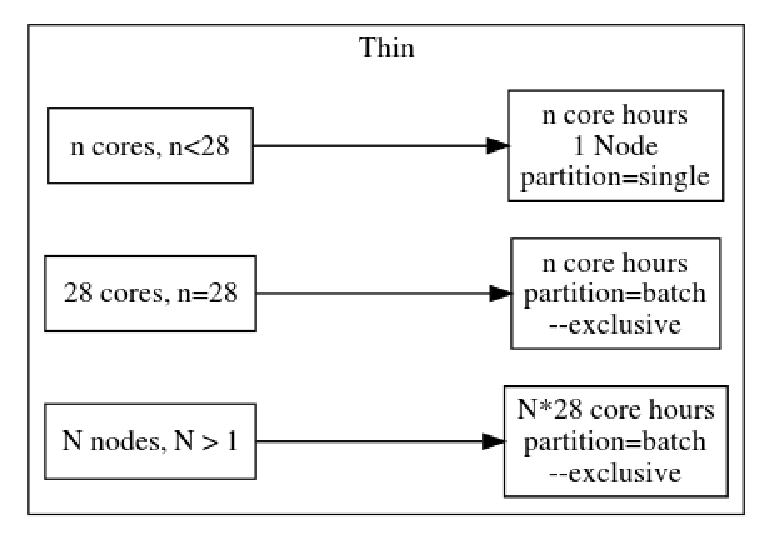
\includegraphics[width=8.5cm]{images/allokation-thinnode.eps}

                Thin node
        \end{center}

\end{frame}

%%%%%%%%%%%%%%%%% NEW  SLIDE
\begin{frame}
	\frametitle{How resources are charged?}

        \begin{center}
		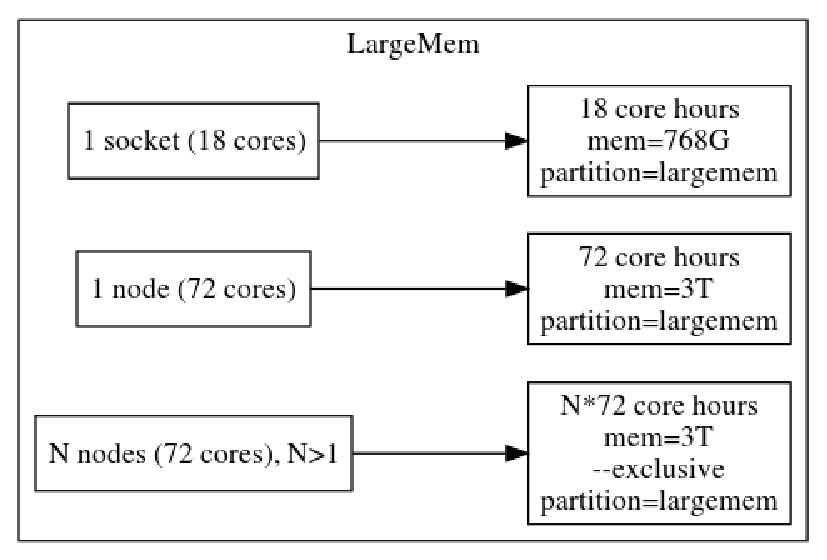
\includegraphics[width=8.5cm]{images/allokation-fatnode.eps}

                Fat node
        \end{center}

\end{frame}

%%%%%%%%%%%%%%%%% NEW  SLIDE
\begin{frame}
	\frametitle{How resources are charged?}

        \begin{center}
		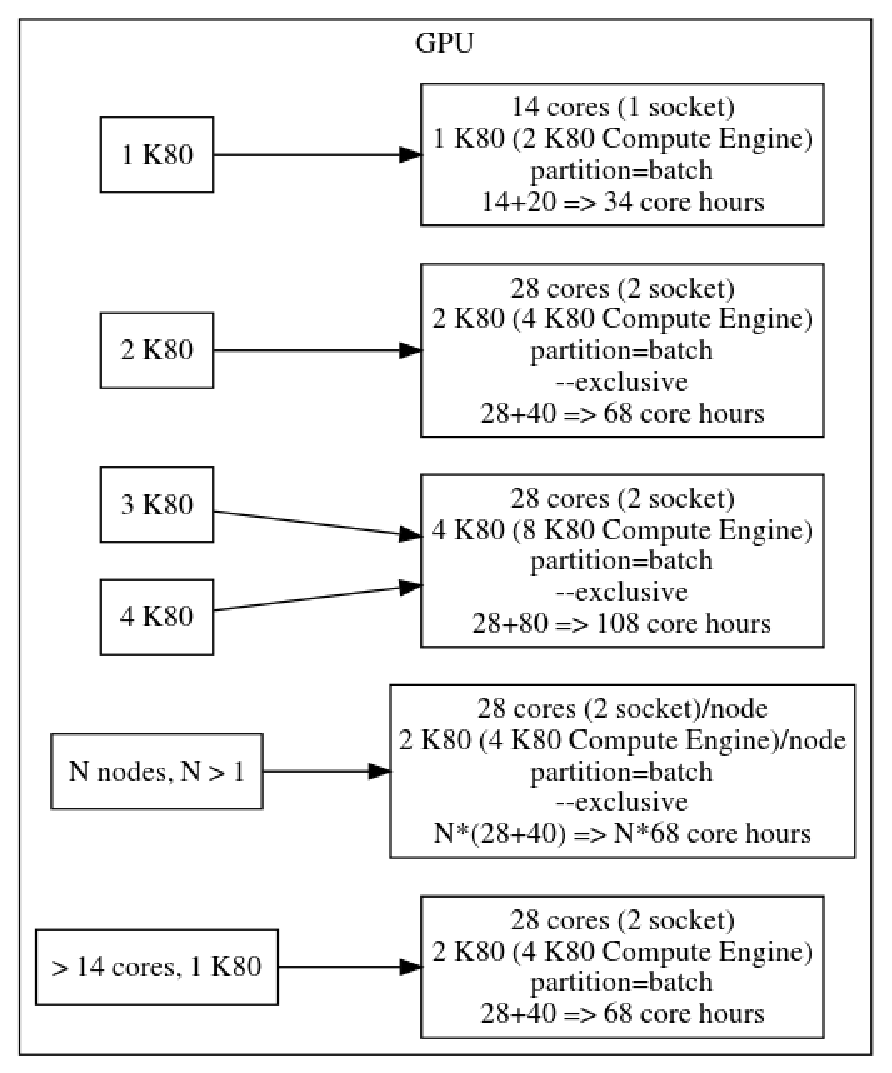
\includegraphics[width=5.7cm]{images/allokation-gpu.eps}

                GPU node
        \end{center}

\end{frame}


%------------------  NEW SUBSECTION ------------------
\subsection{Connecting}

%%%%%%%%%%%%%%%%% NEW  SLIDE
\begin{frame}
	\frametitle{Connecting from a Windows System}

	You need an ssh client to connect.
	\begin{itemize}
		\item	PuTTY
		\item	Cygwin
	\end{itemize}

	If you want to open graphical displays, you need an X11 server
	\begin{itemize}
		\item	Xming
		\item	Cygwin
	\end{itemize}

	Transferring files (sftp or scp)
	\begin{itemize}
		\item	WinSCP
		\item	FileZilla (only sftp)
		\item	PSCP/PSFTP
	\end{itemize}

\end{frame}

%%%%%%%%%%%%%%%%% NEW  SLIDE
\begin{frame}
	\frametitle{Connecting from a UNIX/Linux System}

	\begin{itemize}
		\item	Login with ssh:\\
		 \texttt{local> ssh username@abisko.hpc2n.umu.se}
		\item	If you want to open graphical displays, you need
				to enable X11 Forwarding:\\
		 \texttt{local> ssh -X username@abisko.hpc2n.umu.se}
		\item	Use scp for file transfer:\\
		 \texttt{local> scp username@abisko.hpc2n.umu.se:file /tmp}\\
		 \texttt{local> scp file username@abisko.hpc2n.umu.se:file}
	\end{itemize}

\end{frame}

%%------------------  NEW SUBSECTION ------------------
\subsection{GROMACS}

\begin{frame}[fragile]
	\frametitle{GROMACS}
  
        \begin{verbatim}             
$module spider GROMACS/2016-hybrid 
------------------------------------------------------------------------------------------------------------------------------------------------------------------------------------------------------------------------------------------------------------------
  GROMACS: GROMACS/2016-hybrid
------------------------------------------------------------------------------------------------------------------------------------------------------------------------------------------------------------------------------------------------------------------
 Description:
   GROMACS is a versatile package to ... 
   Homepage: http://www.gromacs.org 

   You will need to load all module(s) on any one of 
   the lines below before the "GROMACS/2016-hybrid" ...

   GCC/5.4.0-2.26  CUDA/8.0.44  OpenMPI/2.0.1
   GCC/6.2.0-2.27  OpenMPI/2.0.1

        \end{verbatim}

\end{frame}


%%%%%%%%%%%%%%%%% NEW  SLIDE
\begin{frame}[fragile]
	\frametitle{GROMACS batch script}
  
        \begin{verbatim}             
#!/bin/bash
#SBATCH -A ~SNICYYYY-XX-NN
#SBATCH -J G2016-gpu
#SBATCH -t 01:00:00
#SBATCH -n 12
#SBATCH -c 7
#SBATCH --gres=gpu:k80:2
#SBATCH -p batch
module add CUDA/8.0.44   GCC/5.4.0-2.26   
module add OpenMPI/2.0.1 GROMACS/2016-hybrid
mdargs="-ntomp $SLURM_CPUS_PER_TASK"
mpirun -np $SLURM_NTASKS gmx_mpi mdrun $mdargs \ 
-dlb yes  -v -deffnm npt
        \end{verbatim}

\end{frame}



%%%%%%%%%%%%%%%%% NEW  SLIDE
\begin{frame}[fragile]
	\frametitle{GROMACS output}
  
        \begin{verbatim}             
    
Running on 3 nodes with total 84 cores, 
84 logical cores, 12 compatible GPUs
  Cores per node:           28                                          
  Logical cores per node:   28                 
  Compatible GPUs per node:  4                 
  All nodes have identical type(s) of GPUs  

        \end{verbatim}

\end{frame}
%%%%%%%%%%%%%%%%% NEW  SLIDE
\begin{frame}
	\frametitle{GROMACS performance 100K atoms}
        \begin{center}
		\includegraphics[width=8.5cm]{images/data_kebne.eps}
        \end{center}
\end{frame}



%########################  NEW SECTION  ########################
%% Section: Using Abisko
% Latex file for the MPI Course at HPC2N Umea 
%    Elaborated by P. Ojeda
%

%########################  NEW SECTION  ########################
\section{Using Abisko}

%%%%%%%%%%%%%%%%% NEW  SLIDE
\begin{frame}
	\frametitle{Abisko}
\includegraphics[width=4.5cm]{images/kebnekeise.eps}
	\begin{itemize}
		\item	332 nodes/15936 cores
		\item	10 fat nodes (512 GB RAM), 318 thin nodes (128 GB RAM)
		\item	CPUs: (thin) 4 x AMD Opteron 6238 (Interlagos) 12 core (2.6 GHz)
		\item	CPUs: (fat) 4 x AMD Opteron 6344 (Abu Dhabi) 12 core (2.6 GHz)
		\item	Interconnect: Infiniband QDR, 40Gb/s, Mellanox
		\item	Installed 2011
	\end{itemize}
\end{frame}




%########################  NEW SECTION  ########################
%% Section: Hands On
% Latex file for the MPI Course at HPC2N Umea 
%    Elaborated by P. Ojeda
%

%########################  NEW SECTION  ########################
\section{Hands-on}



%%%%%%%%%%%%%%%%% NEW  SLIDE
\begin{frame}
	\frametitle{Simple hands-on}
  
	\begin{enumerate}
		\item	Log in to Abisko.
		\item	Go to the parallel file system.
		\item	Copy executable (threaded program)and submit file:\\
				\texttt{cp \~{}mr/Public/mandel .}\\
				\texttt{cp \~{}mr/Public/submit .}
		\item	Put the submit file into the batch queue.
		\item	Look at the queue.
		\item	Where did the output from the program go?
		\item	Run on 12 cores instead.
				Does it run twice as fast?
		\item	The program creates a picture on a file (\texttt{mandel.ppm})
				as output.
				Try looking at it (e.g. using the command \texttt{display}).
	\end{enumerate}

\end{frame}





\end{document}
